\documentclass[11pt]{article}

\usepackage[a4paper,margin=1in]{geometry}
\usepackage{amsmath,amssymb,amsthm,mathtools,tikz}
\usepackage{subcaption}
\usepackage{enumitem}

\newcommand{\LRF}{\mathrm{LRF}}
\newcommand{\OPT}{\mathrm{OPT}}
\newcommand{\maxi}{\max}
\newcommand{\mini}{\min}

\title{Maximums of $\lambda$ for $\alpha \ge \frac12$}
\author{}
\date{}

\begin{document}
Consider the instance $I = \{1,1,p\}$ on $m=2$ machines. 
With schedules: 

\begin{figure}[ht]
\centering
\begin{subfigure}[t]{0.47\textwidth}
\centering
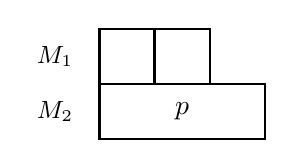
\begin{tikzpicture}[
    x=0.7cm,
    y=0.7cm,
    job/.style={
        draw,
        thick,
        fill=white,
        font=\small
    },
    machine/.style={font=\small}
]

% ------------------------------------------------
% Template idea:
% row      = displayed vertical row in the picture
% machine  = actual machine label shown on the left
%
% Use \machinerow{row}{machine label}
% Use \dotsrow{row}
% Use \jobblock{row}{start}{length}{job label}
% Use \jobblock[gray!25]{row}{start}{length}{job label} for shading
% ------------------------------------------------

\newcommand{\machinerow}[2]{
    \node[machine, anchor=east] at (-0.3,-#1+0.5) {$M_{#2}$};
}

\newcommand{\dotsrow}[1]{
    \foreach \dy in {-0.18,0,0.18} {
        \fill (-0.6,{-#1+0.5+\dy}) circle[radius=0.025];
        \fill (2,{-#1+0.5+\dy}) circle[radius=0.025];
    }
}

\newcommand{\jobblock}[5][white]{
    \draw[job, fill=#1] (#3,-#2) rectangle ++(#4,1);
    \node at ({#3 + #4/2},{-#2 + 0.5}) {$#5$};
}

% Displayed machine rows
\machinerow{1}{1}
\machinerow{2}{2}



% Example jobs
\jobblock{1}{0}{1}{}
\jobblock{1}{1}{1}{}
\jobblock{2}{0}{3}{p}



\end{tikzpicture}

\caption{$S_{OPT}$}
\label{fig:instance-43-opt}
\end{subfigure}
\hfill
\begin{subfigure}[t]{0.47\textwidth}
\centering
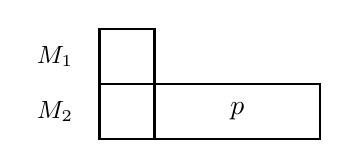
\begin{tikzpicture}[
    x=0.7cm,
    y=0.7cm,
    job/.style={
        draw,
        thick,
        fill=white,
        font=\small
    },
    machine/.style={font=\small}
]

% ------------------------------------------------
% Template idea:
% row      = displayed vertical row in the picture
% machine  = actual machine label shown on the left
%
% Use \machinerow{row}{machine label}
% Use \dotsrow{row}
% Use \jobblock{row}{start}{length}{job label}
% Use \jobblock[gray!25]{row}{start}{length}{job label} for shading
% ------------------------------------------------

\newcommand{\machinerow}[2]{
    \node[machine, anchor=east] at (-0.3,-#1+0.5) {$M_{#2}$};
}

\newcommand{\dotsrow}[1]{
    \foreach \dy in {-0.18,0,0.18} {
        \fill (-0.6,{-#1+0.5+\dy}) circle[radius=0.025];
        \fill (2,{-#1+0.5+\dy}) circle[radius=0.025];
    }
}

\newcommand{\jobblock}[5][white]{
    \draw[job, fill=#1] (#3,-#2) rectangle ++(#4,1);
    \node at ({#3 + #4/2},{-#2 + 0.5}) {$#5$};
}

% Displayed machine rows
\machinerow{1}{1}
\machinerow{2}{2}



% Example jobs
\jobblock{1}{0}{1}{}
\jobblock{2}{0}{1}{}
\jobblock{2}{1}{3}{p}



\end{tikzpicture}

\caption{$S_{LRF}$}
\label{fig:instance-43-lrf}
\end{subfigure}
\caption{Schedules}
\label{fig:instance-43-ratio}
\end{figure}
Then. 
\begin{align*}
    \lambda(I)(0) \ge \frac{C(S_{\LRF})(0)}{C(S_{\OPT})(0)} =\frac{(p+1)^2-p^2-1}{2}=p
\end{align*}

which is obviously unbounded when increasing $p$. Thus the approximation ratio for $\alpha=0$ is unbounded. 

\end{document}